% This is a sample LaTeX input file.  (Version of 9 April 1986) 
% 
% A '%' character causes TeX to ignore all remaining text on the line, 
% and is used for comments like this one.

\documentclass[html]{article}    % Specifies the document style.
\usepackage{graphicx}
                           % The preamble begins here. 
\usepackage{alltt}
\title{Ontology Engineering \& Semantic Web \\ Project Report}  % Declares the document's title. 
\author{Panagiotis Chatzichristodoulou and Kirill Tumanov}    % Declares the author's name
\date{March 27, 2014}   % Deleting this command produces today's date.

%
\begin{document}           % End of preamble and beginning of text.
%
\maketitle                 % Produces the title.
%
\begin{abstract}
%
This work serves as a reference and a summary document for the designed Student Lifecycle Management (SLM) system ontology, based on the SAP AG framework. It gives an overall structure of the ontology and describes the main functions of student lifecycle it reflects. For better comprehension this description is coupled with following the built-it exemplar individuals. The paper ends with discussion on ontology limitations and possible future work.
%
\end{abstract}
%
% 
\section{Introduction}
%
Ontology engineering is a field that studies the methods and methodologies of building ontologies. From an Artificial Intelligence point of view, an ontology is defined as: ``explicit specification of conceptualization''~\cite{Gruber}, meaning that ontologies are formal representations of sets of concepts and the relations between them within a domain. It must be noted that even though ontologies are build to serve as formal representations of a certain problem, ontologies should be build as problem-independent as possible. Consequently, an ontology about a car of a certain brand must also be able to represent cars of other brads without any modifications. The domain of the ontology described in this paper is the domain of SLM, meaning that the ontology build creates a framework that describes the Student Lifecycle Management system. Despite the fact that it was based on SAP-SLM~\cite{sap}, the ontology can represent a much wider range of student lifecycle management systems.
\\
For the creation of the ontology Protege tool was used. For the visualization and the analysis of the ontology, protege plugins \textit{OntoGraph}~\cite{protegeOntoGraph} and \textit{CloudView}~\cite{protegeCloudViews} were used. The ontology created abides by the \textit{OntoClean}~\cite{ontoCleanPaper} standards.
% 
\section{Implementation}
%
The ontology of SLM system was designed according to the available SAP AG framework, shown in Fig.~\ref{SAP}.
\begin{figure}[htbp]
  \centering
    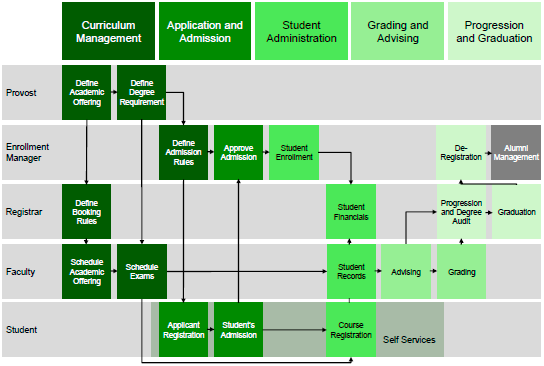
\includegraphics[width=0.8\textwidth]{Materials/Figures/1.png}
    \caption{SAP AG framework of SLM~\cite{sap}}
  \label{SAP}
\end{figure}

%
% ---- Bibliography ----
%
\begin{thebibliography}{99}
%
\bibitem {sap}
Solution in Detail: Higher Education and Research. Student Life Management.
SAP AG, \texttt{http://www.sap.com/bin/sapcom/en\_us/downloadasset.2013-12-dec\newline-11-11.higher-education-and-research-student-lifecycle-\newline management-pdf.html}(2013)

\bibitem{protege}
Protege ontology creation tool Website.\\
\texttt{http://protege.stanford.edu/}

\bibitem{protegeWiki}
Protege ontology creation tool Wiki.\\
\texttt{http://protegewiki.stanford.edu/wiki/Main\_Page}

\bibitem{protegeCloudViews}
Protege tool cloud views plugin.\\
\texttt{http://protegewiki.stanford.edu/wiki/Cloud\_Views}

\bibitem{protegeOntoGraph}
Protege onto graph views plugin.\\
\texttt{http://protegewiki.stanford.edu/wiki/OntoGraf}

\bibitem{ontoCleanPaper}
Ontoclean Method.\\
\texttt{http://www.researchgate.net/publication/27293101\_Evalu-\newline
ating\_ontological\_decisions\_with\_OntoClean/file/9fcfd50-\newline
f9621161392.pdf}

\bibitem{Gruber}
Gruber T.:
\\
\texttt{http://www-ksl.stanford.edu/kst/ what-is-an-ontology.html.} 



%%%%%%%%%%%%%%%%%%%%%%%%%%%%%%%%%%%%%%%%%%%%%%%%%%%%%%%%%%%%%%%%%%%
\end{thebibliography}
\end{document}             % End of document. 